\documentclass[usepdftitle=false,aspectratio=169,usenames,dvipsnames]{beamer}
\usepackage{amsmath, amsfonts, amssymb}
\usepackage{algorithm}
\usepackage[noend]{algpseudocode}
\usepackage{xspace}
\usepackage{xparse}
\usepackage[yyyymmdd]{datetime}
\usepackage{ulem}
\usepackage{array}
\usepackage{listings}
\usepackage{multirow}
\usepackage{booktabs}
\usepackage{stmaryrd}
\usepackage{caption}
\usepackage{subcaption}
\usepackage{bussproofs}
\usepackage{mathpartir}
\usepackage{minted}
\usepackage{xcolor}
\usepackage{proof}
\usepackage{tcolorbox}
\usepackage{relsize}
\usepackage{comment}

\usepackage{tikz}
\usetikzlibrary{shapes.geometric, arrows.meta}
\tcbuselibrary{raster}
\captionsetup{font=tiny}
\definecolor{keywordcolor}{rgb}{0.7, 0.1, 0.1}
\definecolor{tacticcolor}{rgb}{0.0, 0.1, 0.6}
\definecolor{commentcolor}{rgb}{0.4, 0.4, 0.4}
\definecolor{symbolcolor}{rgb}{0.0, 0.1, 0.6}
\definecolor{sortcolor}{rgb}{0.1, 0.5, 0.1}
\definecolor{attributecolor}{rgb}{0.7, 0.1, 0.1}
\usetikzlibrary{shapes,arrows,positioning,decorations.markings,matrix,fit,calc}
\tikzstyle{line} = [draw, -latex']
\tikzstyle{rline} = [draw, latex'-]
\pgfdeclarelayer{background}
\pgfsetlayers{background,main}
\EnableBpAbbreviations

\DeclareUnicodeCharacter{2081}{$_{1}$}
\DeclareUnicodeCharacter{03B1}{$\alpha$}
\DeclareUnicodeCharacter{2200}{$\mathbb{\forall}$}
\DeclareUnicodeCharacter{2203}{$\mathbb{\exists}$}

\DeclareUnicodeCharacter{2265}{$\ge$}
\DeclareUnicodeCharacter{2227}{$\wedge$}
\DeclareUnicodeCharacter{2243}{$\simeq$}
\DeclareUnicodeCharacter{2264}{$\mathbb{\le}$}
\DeclareUnicodeCharacter{2228}{$\vee$}
\DeclareUnicodeCharacter{2084}{$_{4}$}
\DeclareUnicodeCharacter{2083}{$_{3}$}
\DeclareUnicodeCharacter{2082}{$_{2}$}
\DeclareUnicodeCharacter{208A}{$_{+}$}
\DeclareUnicodeCharacter{1D62}{$_{i}$}
\DeclareUnicodeCharacter{208B}{$_{-}$}

\hypersetup{
  pdftitle={Automating Elementary Number-theoretic Proofs using Gr\"obner Bases},
  pdfauthor={Tomaz Mascarenhas},
  pdfkeywords={},
  pdfborder={0 0 0},
  draft=false,
  bookmarksnumbered,
  bookmarksdepth=2,
  bookmarksopenlevel=2,
  bookmarksopen
}

\renewcommand{\dateseparator}{--}

%%% BEGIN Defining style
\useinnertheme[outline]{chamfered}
\setbeamertemplate{navigation symbols}{}
\usefonttheme[onlymath]{serif}
\usecolortheme{seahorse}
\setbeamercolor{palette quinary}{use=structure,fg=black,bg=white}
%%% END Defining style

%%% BEGIN Biblatex for references
\usepackage[backend=bibtex,
doi=false,isbn=false,url=false,
style=alphabetic,
maxalphanames= 4, maxcitenames = 3, minalphanames = 3, minnames = 3]{biblatex}

\bibliography{./refs.bib}

\mathchardef\mhyphen="2D

\usepackage{pifont}

\newcommand{\bluecheck}{{\color{blue}\checkmark}}
\newcommand{\greencheck}{{\color{blue}\checkmark}}
\newcommand{\redmark}{\color{red}{\ding{55}}}

\newcommand\vitem{\vfill\item}
\newcommand\pvitem{\pause\vfill\item}
\newcommand\pitem{\pause\item}

% Algebra and number theory
\newcommand{\Id}{\operatorname{Id}}
\newcommand{\coprime}{\operatorname{coprime}}
\newcommand{\divides}{\operatorname{divides}}
\newcommand{\congruent}{\operatorname{congruent}}

\setbeamertemplate{frametitle continuation}{}
\renewcommand*{\bibfont}{\scriptsize}
%%% END Biblatex for references

%%% BEGIN DEFINING TITLE PAGE

\defbeamertemplate{title page}{mystyle}[1][]
{
  \vbox{}
  \vfill
  \begingroup
    \centering
    {\usebeamercolor[fg]{titlegraphic}\inserttitlegraphic\par}
    \vskip1em
    % The chamfered theme places the text 2*(corners+padding) = 8pt to the right of
    % where beamercolorbox expects, so we center it on 8pt less to keep it centered.
    \begin{beamercolorbox}[sep=0pt,leftskip=0pt plus1fill,rightskip=8pt plus1fill,#1,rounded=true,wd=12cm]{title}
      \usebeamerfont{title}\inserttitle\par%
      \ifx\insertsubtitle\@empty%
      \else%
        \vskip0.25em%
        {\usebeamerfont{subtitle}\usebeamercolor[fg]{subtitle}\insertsubtitle\par}%
      \fi%
    \end{beamercolorbox}%
    \vskip1em\par
    \begin{beamercolorbox}[sep=8pt,center,#1]{author}
      \usebeamerfont{author}\insertauthor
    \end{beamercolorbox}
  \endgroup
  \vfill
}

\setbeamertemplate{title page}[mystyle]

\date{Theory and Practice of SMT Solving, UFMG, 2026}
%%% END DEFINING TITLE PAGE

%%% BEGIN Meta information

\author[Tomaz Mascarenhas]
{%
  \texorpdfstring{
      Tomaz Mascarenhas \\ \vspace{1ex} {\footnotesize Original paper by John Harrison (CADE 2007)}
      \vspace{3ex}
    \begin{columns}
      \column{.45\linewidth}
        \centering
        
\includegraphics[height=0.25\textheight]{images/DCC_LOGO.jpg}
      \column{.35\linewidth}
        
\includegraphics[height=0.15\textheight]{images/Logo_UFMG.jpg}
    \end{columns}
  }
  {}
}

\title[Number-theoretic Proofs using Gr\"obner Bases]{Automating Elementary Number-theoretic Proofs using Gr\"obner Bases}

\makeatother
\setbeamertemplate{footline}
{
  \leavevmode%
  \hbox{%
    \begin{beamercolorbox}[wd=.6\paperwidth,ht=2.5ex,dp=1ex,left]{title in head/foot}%
      {\hspace{1em}\usebeamerfont{title in head/foot}\insertshorttitle}
    \end{beamercolorbox}%
    \begin{beamercolorbox}[wd=.2\paperwidth,ht=2.5ex,dp=1ex,left]{title in head/foot}%
      {\hspace{1em}\usebeamerfont{title in head/foot}Tomaz Mascarenhas, UFMG}
    \end{beamercolorbox}%
    \begin{beamercolorbox}[wd=.2\paperwidth,ht=2.5ex,dp=1ex,right]{title in head/foot}%
      \insertframenumber{} / \inserttotalframenumber\hspace{1em}
    \end{beamercolorbox}}%
  \vskip0pt%
}
\makeatletter
%%% END Meta information

%%% BEGIN Tikz setup
\usepackage{tikz}
\usetikzlibrary{positioning,calc,intersections,backgrounds, fadings}
\usetikzlibrary{shapes}

  \tikzset{
    invisible/.style={opacity=0},
    visible on/.style={alt=#1{}{invisible}},
    alt/.code args={<#1>#2#3}{%
      \alt<#1>{\pgfkeysalso{#2}}{\pgfkeysalso{#3}}
    },
  }

\definecolor{BloodRed}{rgb}{.86,0,0}
\definecolor{ao}{rgb}{0.0, 0.0, 1.0}
\definecolor{ao(english)}{rgb}{0.0, 0.5, 0.0}
\definecolor{ceruleanblue}{rgb}{0.16, 0.32, 0.75}
%%% END Tikz setup

\usepackage{soul,xcolor}
\setstcolor{red}

\AtBeginSection[]{
  {
    \setbeamertemplate{footline}{}
  \begin{frame}
  \vfill
  \centering
  \begin{beamercolorbox}[sep=8pt,center,shadow=true,rounded=true]{title}
    \usebeamerfont{title}\insertsectionhead\par%
  \end{beamercolorbox}
  \vfill
\end{frame}
}
\addtocounter{framenumber}{-1}
}

\addtobeamertemplate{theorem begin}{%
  \setbeamercolor{block title}{fg=white,bg=black}%
  \setbeamercolor{block body}{fg=black, bg=white!90!black}%
}{}

%%% BEGIN CHANGING BULLETS STYLE
\setbeamertemplate{itemize item}{$\vartriangleright$}
\setbeamertemplate{itemize subitem}{$\blacktriangleright$}
\setlength\leftmargini{1em}
\setlength\leftmarginii{1.25em}
\setlength\leftmarginiii{1em}
%%% END CHANGING BULLETS STYLE

\setbeamersize{text margin left=1em, text margin right=1.5em}

\newcommand{\red}[1]{\textcolor{red}{#1}}

%%% BEGIN Review boxes (strengths and weaknesses of the paper)
\newtcolorbox{strengthbox}{colback=blue!4, colframe=blue!50!black, boxrule=0.5pt,
  arc=2pt, left=4pt, right=4pt, top=2pt, bottom=2pt}
\newtcolorbox{weaknessbox}{colback=red!4, colframe=red!50!black, boxrule=0.5pt,
  arc=2pt, left=4pt, right=4pt, top=2pt, bottom=2pt}
\newcommand{\strength}[1]{\begin{strengthbox}\small\bluecheck\ \textbf{Strength:} #1\end{strengthbox}}
\newcommand{\weakness}[1]{\begin{weaknessbox}\small{\redmark}\ \textbf{Weakness:} #1\end{weaknessbox}}
%%% END Review boxes

\begin{document}

{
\setbeamertemplate{footline}{}
\frame{\titlepage}
}
\addtocounter{framenumber}{-1}

\begin{frame}
  \frametitle{A Motivating Example}
  \begin{itemize}
    \item Cancellation law for congruences:
  \end{itemize}
  \begin{tcolorbox}[colback=green!5,colframe=green!40!black,title=Example]
    \centering
    $\forall a\, n\, x\, y \in \mathbb{Z} .\;\; \congruent(ax, ay, n) \;\wedge\; \coprime(a, n) \;\Rightarrow\; \congruent(x, y, n)$
  \end{tcolorbox}
  \begin{itemize}
    \vitem Nonlinear integer arithmetic augmented with number-theoretic predicates:
      \vspace{4pt}

      \hspace{2em}
      \begin{tabular}{@{$\blacktriangleright$\;}l@{\hspace{2em}}l}
        $\divides(s, t)$ & $s$ divides $t$ \\
        $\congruent(s, t, u)$ & $s$ is congruent to $t$ modulo $u$ ($s \equiv t \text{ (mod u)}$) \\
        $\coprime(s, t)$ & $s$ and $t$ have no common factor
      \end{tabular}
    \pvitem Neither cvc5 nor z3 solve the SMT-LIB encoding of the problem above within 1 minute.
  \end{itemize}
\end{frame}

\begin{frame}
  \frametitle{Applications}
  \begin{itemize}
    \item Verification of programs using \texttt{div} and \texttt{mod} with a \textbf{non-constant} divisor
      \begin{itemize}
        \item e.g.\ verification conditions generated by Verus, Dafny, F$^\star$
      \end{itemize}
    \pvitem Bit-vectors of symbolic width $k$, translated to integers: arithmetic modulo $2^k$
      \[ \mathtt{bvadd}_k(x, y) \;\rightsquigarrow\; (x + y) \bmod 2^k \]
    \pvitem Harrison's original motivation: routine divisibility lemmas in proof assistants (HOL Light)
  \end{itemize}
\end{frame}

\begin{frame}
  \frametitle{State of the Art}
  \begin{itemize}
    \item The predicates can be encoded with fresh variables, e.g.\ $\divides(s, t) \;\rightsquigarrow\; \exists d.\; t = sd$
    \pvitem The result is nonlinear even for problems that originally don't contain multiplication.
      \begin{itemize}
        \item General techniques: incremental linearization, cylindrical algebraic coverings with branch and bound \ldots
      \end{itemize}
    \pvitem There is currently no method designed for handling divisibility constraints.
  \end{itemize}
  \pause
  \vfill
  \strength{real progress on a problem with many applications, which is not well explored.}
\end{frame}

% Overview of the method. Each step is revealed with an overlay.
\begin{frame}
  \frametitle{Harrison's Method}
  \begin{itemize}
    \item Uniform procedure for formulas with $+$, $-$, $\times$, $\divides$, $\congruent$, $\coprime$ and a limited quantifier structure
    \vitem Reduces the problem to \textbf{ideal membership}, decided with \textbf{Gr\"obner bases}
    \vitem Sound but incomplete over $\mathbb{Z}$; complete for properties that hold in \textbf{every commutative ring}
    \vitem Implemented in the HOL Light proof assistant
  \end{itemize}
  \vfill
  \centering
  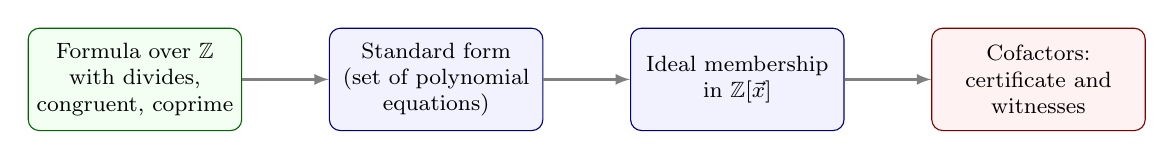
\begin{tikzpicture}[
      box/.style={draw, rounded corners, align=center, inner sep=3pt, text width=2.5cm, minimum height=1.3cm, font=\footnotesize},
      arr/.style={-latex, thick, gray},
      lab/.style={font=\scriptsize, text=gray!60!black, align=center}
    ]
    \node[box, draw=green!40!black, fill=green!5] (f) {Formula over $\mathbb{Z}$ \\ with $\divides$, \\ $\congruent$, $\coprime$};
    \node[box, draw=blue!50!black, fill=blue!5, right=1.1cm of f, visible on=<2->] (s) {Standard form \\ (set of polynomial equations)};
    \node[box, draw=blue!50!black, fill=blue!5, right=1.1cm of s, visible on=<3->] (i) {Ideal membership \\ in $\mathbb{Z}[\vec{x}]$};
    \node[box, draw=red!50!black, fill=red!5, right=1.1cm of i, visible on=<4->] (c) {Cofactors: \\ certificate and witnesses};
    \draw[arr, visible on=<2->] (f) -- node[lab, above] {} (s);
    \draw[arr, visible on=<3->] (s) -- node[lab, above] {} (i);
    \draw[arr, visible on=<4->] (i) -- node[lab, above] {} (c);
  \end{tikzpicture}
\end{frame}

\begin{frame}
  \frametitle{Outline}
  \begin{itemize}
    \item Introduction \bluecheck
    \vitem Harrison's Method
    \vitem Implementation and Evaluation
    \vitem My Project: Harrison's Method in cvc5
  \end{itemize}
\end{frame}

\section{Harrison's Method}

\begin{frame}
  \frametitle{Step 1: Expanding the Predicates}
  \begin{itemize}
    \item Each predicate abbreviates an existential formula:
  \end{itemize}
  \[
    \begin{array}{rcl}
      \divides(s, t) & := & \exists d.\; t = sd \\
      \congruent(s, t, u) & := & \exists d.\; t - s = ud \\
      \coprime(s, t) & := & \exists x\, y.\; sx + ty = 1
    \end{array}
  \]
  \vfill
  \onslide<2->{
  \begin{tcolorbox}[colback=green!5,colframe=green!40!black,title=Example]
    $\forall a\, n\, x\, y.\;\; \congruent(ax, ay, n) \;\wedge\; \coprime(a, n) \;\Rightarrow\; \congruent(x, y, n)$
    \\[4pt]
    \onslide<3->{$\rightsquigarrow\; \forall a\, n\, x\, y.\;\; (\exists d.\; ay - ax = nd) \;\wedge\; (\exists u\, v.\; au + nv = 1) \;\Rightarrow\; \exists k.\; y - x = nk$}
    \\[4pt]
    \onslide<4->{$\rightsquigarrow\; \forall a\, n\, x\, y\, \red{d\, u\, v}.\;\; ay - ax = nd \;\wedge\; au + nv = 1 \;\Rightarrow\; \exists k.\; y - x = nk$}
  \end{tcolorbox}
  }
  \onslide<4->{\small The existentials in the hypotheses become universal variables (prenex form).}
\end{frame}

\begin{frame}
  \frametitle{Standard Form}
  \begin{itemize}
    \item Target: formulas of the form
  \end{itemize}
  \[
    \forall \vec{x}.\;\; \bigwedge_{i=1}^{m} e_i(\vec{x}) = 0 \;\Rightarrow\; \exists y_1 \cdots y_n.\;\;
    \begin{array}[t]{@{}l@{}}
      p_{11}(\vec{x})\, y_1 + \cdots + p_{1n}(\vec{x})\, y_n = a_1(\vec{x}) \;\wedge \\
      \qquad \cdots \;\wedge \\
      p_{k1}(\vec{x})\, y_1 + \cdots + p_{kn}(\vec{x})\, y_n = a_k(\vec{x})
    \end{array}
  \]
  \begin{itemize}
    \item Hypotheses: polynomial equations. Conclusion: $k$ equations, each \textbf{linear} in the $y_j$
    \pvitem Divisibility constraints are encoded with existential variables, thus they naturally fall into this form.
    \pvitem From now on, $k = 1$: we write $p_j$ for $p_{1j}$ and $a$ for $a_1$
  \end{itemize}
  \pause
  \vfill
  \begin{tcolorbox}[colback=green!5,colframe=green!40!black,title=Example]
    \centering
    $\forall a\, n\, x\, y\, d\, u\, v.\;\; \underbrace{ay - ax - nd}_{e_1} = 0 \;\wedge\; \underbrace{au + nv - 1}_{e_2} = 0 \;\Rightarrow\; \exists k.\;\; \underbrace{n}_{p_1} k = \underbrace{y - x}_{a}$
  \end{tcolorbox}
\end{frame}

\begin{frame}
  \frametitle{Step 2: The Key Idea}
  \begin{tcolorbox}[colback=green!5,colframe=green!40!black,title=Example,top=1pt,bottom=1pt,after skip=6pt]
    \centering
    $\forall a\, n\, x\, y\, d\, u\, v.\;\; \underbrace{ay - ax - nd}_{e_1} = 0 \;\wedge\; \underbrace{au + nv - 1}_{e_2} = 0 \;\Rightarrow\; \exists k.\;\; \underbrace{n}_{p_1} k = \underbrace{y - x}_{a}$
  \end{tcolorbox}
  \begin{itemize}
    \item Idea: find \textbf{polynomials} $c_1$, $c_2$, $c_3$ that make the following a polynomial identity:
      \[ a \;=\; c_1 \cdot e_1 \;+\; c_2 \cdot e_2 \;+\; c_3 \cdot p_1 \]
  \end{itemize}
  \onslide<2->{
  \begin{tcolorbox}[colback=blue!5,colframe=blue!50!black,title=Solution,top=1pt,bottom=1pt]
    \centering
    $y - x \;=\; \textcolor<3->{gray}{\underbrace{u}_{c_1} \cdot\, (ay - ax - nd)} \;+\; \textcolor<3->{gray}{\underbrace{(x - y)}_{c_2} \cdot\, (au + nv - 1)} \;+\; \underbrace{\textcolor{blue}{(ud + vy - vx)}}_{c_3} \cdot\, n$
  \end{tcolorbox}
  }
  \begin{itemize}
    \item<3-> When the hypotheses hold, $e_1 = e_2 = 0$, and all that is left is $y - x = c_3 \cdot n$
    \item<4-> Thus $k := \textcolor{blue}{ud + vy - vx}$ is a witness.
  \end{itemize}
\end{frame}

\begin{frame}
  \frametitle{Step 2: Ideal Membership}
  \begin{itemize}
    \item The set of all such combinations of $g_1, \dots, g_r$ is the \textbf{ideal} generated by them:
      \[ \langle g_1, \dots, g_r \rangle = \{\, c_1 g_1 + \dots + c_r g_r \;\mid\; c_i \in \mathbb{Z}[\vec{x}] \,\} \]
    \pvitem Test for the standard form: \quad $a \in \langle e_1, \dots, e_m, p_1, \dots, p_n \rangle$
      \begin{itemize}
        \item In the example: \quad $y - x \in \langle\, ay - ax - nd,\;\; au + nv - 1,\;\; n \,\rangle$
      \end{itemize}
    \pvitem Sound: if $a = \sum_i f_i\, e_i + \sum_j g_j\, p_j$, then whenever all $e_i(\vec{x}) = 0$,
      \[ a(\vec{x}) = \textstyle\sum_j g_j(\vec{x})\, p_j(\vec{x}) \]
      so the $g_j(\vec{x})$ are witnesses for the $y_j$
  \end{itemize}
\end{frame}

\begin{frame}
  \frametitle{Deciding Ideal Membership}
  \begin{itemize}
    \item Buchberger's algorithm computes a \textbf{Gr\"obner basis} $G$ of the ideal
      \begin{itemize}
        \item For $n$ variables it takes $\mathcal{O}(2^{2^n})$ steps, but it works well in practice.
      \end{itemize}
    \vitem $a$ is in the ideal iff $a$ reduces to $0$ by repeated division by elements of $G$
    \vitem Recording the reductions gives the cofactors: a \textbf{certificate}
    \vitem Checking it amounts to checking a polynomial identity, by normalizing both sides
      \begin{itemize}
        \item HOL Light translates it into primitive inferences: the Gr\"obner basis code is not trusted
      \end{itemize}
  \end{itemize}
  \pause
  \vfill
  \strength{easily certifiable, which is essential in formal verification. Checking is much cheaper than solving.}
\end{frame}

\begin{frame}
  \frametitle{Sound but Incomplete}
  \begin{itemize}
    \item Over $\mathbb{Z}$, no test of this kind can be both sound and complete:
      \begin{itemize}
        \item Special case: $\forall \vec{x}.\; \bigwedge_i e_i(\vec{x}) = 0 \Rightarrow \bot$, i.e.\ a Diophantine equation has no solution: undecidable
        \item Ideal membership in $\mathbb{Z}[\vec{x}]$ is decidable (Aschenbrenner, 2004)
      \end{itemize}
    \pvitem Example: $x^2 + x$ is always even
      \[ \forall x.\; \exists k.\; x^2 + x = 2k \quad \text{holds in } \mathbb{Z}, \quad \text{but} \quad x^2 + x \notin \langle 2 \rangle \]
  \end{itemize}
\end{frame}

\begin{frame}
  \frametitle{Completeness over All Rings}
  \begin{itemize}
    \item Even though the method is not complete, the author proves that it can decide formulas that do not depend on properties specific to the integers:
  \end{itemize}
  \pause
  \vfill
  \begin{theorem}
    \abovedisplayskip=3pt \belowdisplayskip=3pt
    Let $e_i, p_j, a \in \mathbb{Z}[\vec{x}]$, and let $\varphi$ be the following sentence:
    \[
      \varphi \;:=\; \forall \vec{x}.\;\; \textstyle\bigwedge_{i=1}^{m} e_i(\vec{x}) = 0 \;\Rightarrow\; \exists y_1 \cdots y_n.\;\; p_1(\vec{x})\, y_1 + \cdots + p_n(\vec{x})\, y_n = a(\vec{x})
    \]
    \[
      \text{Then} \qquad T_{\mathrm{CR}} \models \varphi
      \quad\Longleftrightarrow\quad
      a \in \langle e_1, \dots, e_m, p_1, \dots, p_n \rangle \;\text{ in }\; \mathbb{Z}[\vec{x}]
    \]
  \end{theorem}
  {\footnotesize $T_{\mathrm{CR}}$: theory of commutative rings with unity. $T_{\mathrm{CR}} \models \varphi$ means that $\mathcal{R} \models \varphi$ for every such ring $\mathcal{R}$.}
  \pause
  \vfill
  \strength{interesting theoretical result: the method is principled and predictable, not just a heuristic.}
  \pause
  \weakness{How often do formulas hold in all rings? The author doesn't explore this question}
\end{frame}

\section{Implementation and Evaluation}

\begin{frame}[fragile]
  \frametitle{Implementation in HOL Light}
  \begin{itemize}
    \item Fewer than 100 lines, part of HOL Light since version 2.20
    \item Proves all examples of the paper, e.g.\ a generalization of the Chinese Remainder Theorem:
  \end{itemize}
  \vfill
  \begin{lstlisting}[basicstyle=\ttfamily\footnotesize, columns=fullflexible, keepspaces=true, xleftmargin=1em]
# INTEGER_RULE
   `!a1 a2 n1 n2:int.
       (a1 == a2) (mod (gcd(n1,n2)))
       ==> ?x. (x == a1) (mod n1) /\ (x == a2) (mod n2)`;;
4 basis elements and 1 critical pairs
5 basis elements and 0 critical pairs
1 basis elements and 0 critical pairs
Translating certificate to HOL inferences
val it : thm =
  |- !a1 a2 n1 n2.
         (a1 == a2) (mod gcd (n1,n2))
         ==> (?x. (x == a1) (mod n1) /\ (x == a2) (mod n2))
  \end{lstlisting}
\end{frame}

\begin{frame}
  \frametitle{Gr\"obner Bases over $\mathbb{Q}$, not $\mathbb{Z}$}
  \begin{itemize}
    \item The theorems are about ideals in $\mathbb{Z}[\vec{x}]$, but the implementation runs Buchberger's algorithm over $\mathbb{Q}[\vec{x}]$
    \pvitem Example: ``every integer is even'', $\forall x.\; \exists k.\; 2k = x$, is false in $\mathbb{Z}$, and indeed $x \notin \langle 2 \rangle$ in $\mathbb{Z}[x]$. But in $\mathbb{Q}[x]$:
      \[ x = \tfrac{x}{2} \cdot 2, \quad \text{so } x \in \langle 2 \rangle, \text{ with the ``witness'' } k = \tfrac{x}{2} \]
    \pvitem Still sound: building the HOL proof fails if a cofactor is not integral. But it may fail on formulas that hold in all rings
    \pvitem The author found ``almost no cases where the distinction mattered''
  \end{itemize}
  \pause
  \vfill
  \weakness{mismatch between the theory ($\mathbb{Z}[\vec{x}]$) and the implementation ($\mathbb{Q}[\vec{x}]$), justified only by anecdotes.}
\end{frame}

\begin{frame}
  \frametitle{Evaluation}
  \begin{itemize}
    \item Only a list of examples: cancellation, Chinese Remainder Theorem, gcd properties, \ldots
    \vitem No systematic evaluation nor comparison with other tools
    \vitem The implementation is a ``simple prototype'', and Gr\"obner bases are doubly exponential in the worst case
  \end{itemize}
  \pause
  \vfill
  \weakness{lack of systematic evaluation: there is only anecdotal evidence that the method is usable in practice.}
\end{frame}

\section{Integrating Harrison's Method in cvc5}

\begin{frame}
  \frametitle{Harrison's Method in cvc5}
  \begin{itemize}
    \item Goal: improve cvc5 on verification conditions with \texttt{div} and \texttt{mod} by non-constant divisors
    \pvitem No predicates to expand: cvc5's preprocessing already introduces the witnesses
      \[ (\mathtt{div}\ s\ n) \rightsquigarrow q \;\text{ with }\; n > 0 \Rightarrow nq \le s < n(q + 1), \qquad (\mathtt{mod}\ s\ n) \rightsquigarrow s - nq \]
    \pvitem New step: for each term $s \bmod n$, run Harrison's test with the equalities asserted:
      \begin{itemize}
        \item If it proves $\divides(n, s)$, we learn the lemma $s \bmod n = 0$
        \item If it proves $\congruent(s, s', n)$ for two such terms, we learn $s \bmod n = s' \bmod n$
      \end{itemize}
  \end{itemize}
  \pause
  \vfill
  \begin{tcolorbox}[colback=green!5,colframe=green!40!black,title=Example]
    \centering
    $ay - ax = nd \;\wedge\; au + nv = 1 \;\wedge\; n > 0 \;\Rightarrow\; (y - x) \bmod n = 0$
  \end{tcolorbox}
\end{frame}

\begin{frame}
  \frametitle{Integration and Results}
  \centering
  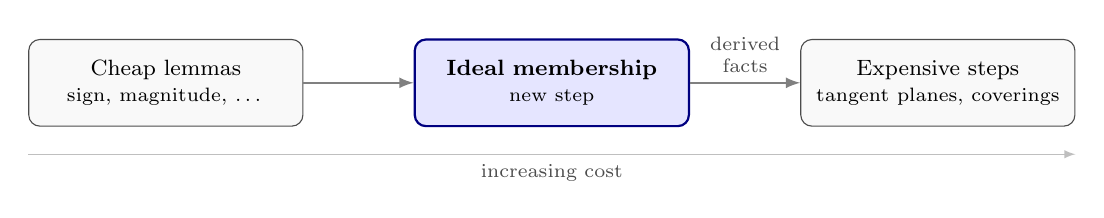
\begin{tikzpicture}[
      box/.style={draw, rounded corners, align=center, inner sep=4pt, text width=3.2cm, minimum height=1.1cm, font=\footnotesize},
      arr/.style={-latex, thick, gray},
      lab/.style={font=\scriptsize, text=gray!60!black, align=center}
    ]
    \node[box, draw=gray!60!black, fill=gray!5] (cheap) {Cheap lemmas \\ \scriptsize sign, magnitude, \ldots};
    \node[box, draw=blue!50!black, fill=blue!10, thick, right=1.4cm of cheap] (ideal) {\textbf{Ideal membership} \\ \scriptsize new step};
    \node[box, draw=gray!60!black, fill=gray!5, right=1.4cm of ideal] (exp) {Expensive steps \\ \scriptsize tangent planes, coverings};
    \draw[arr] (cheap) -- (ideal);
    \draw[arr] (ideal) -- node[lab, above] {derived\\facts} (exp);
    \draw[-latex, gray!50] ([yshift=-0.35cm]cheap.south west) -- node[lab, below] {increasing cost} ([yshift=-0.35cm]exp.south east);
  \end{tikzpicture}
  \vfill
  \raggedright
  \begin{itemize}
    \item<2-> Parametric bit-vectors: from $622$ to $662$ solved problems (out of $1693$). Verus: same number of solved problems. We are still improving the implementation
    \vitem<3-> Relation to the paper:
      \begin{itemize}
        \item Same core test, but used to generate lemmas inside an SMT solver, not as a standalone procedure
        \item Same gap: Gr\"obner bases over $\mathbb{Q}$, integrality of the cofactor of $n$ is checked
        \item Evaluation on benchmark sets, which the paper lacks
      \end{itemize}
  \end{itemize}
\end{frame}

\end{document}
